\chapter{Design methodology} \label{ch:designmet}
This chapter will describe a method for traversing between the algortihm domain and architecture domain in the A$^3$ model described in section \vref{sec:a3model} and the blue lines in figure \vref{fig:a3method} shows where this movement occurs.\\

\begin{figure}[ht!]
  \centering
  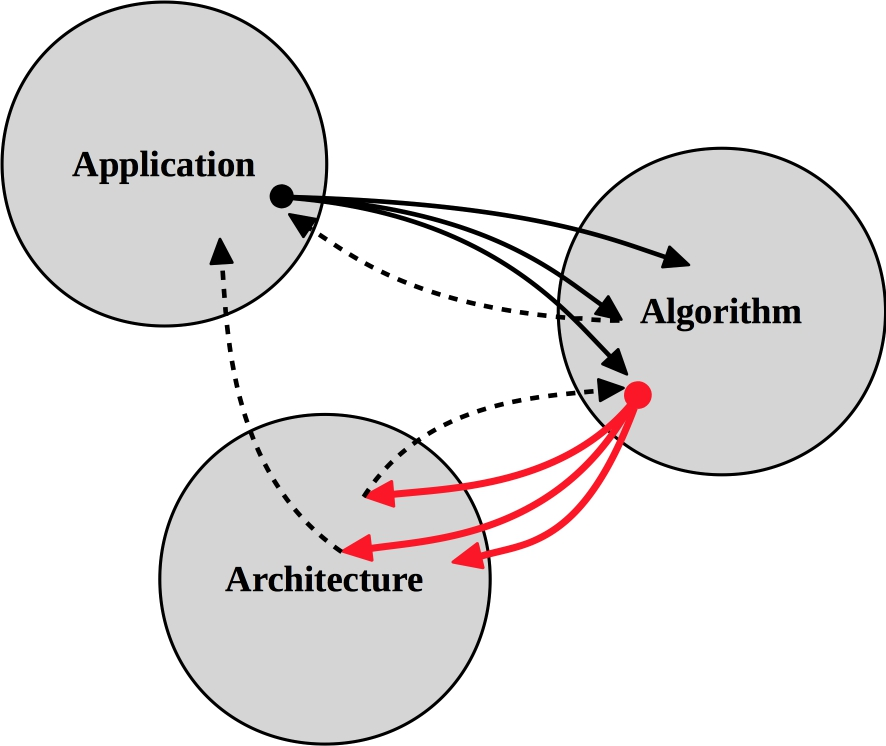
\includegraphics[scale=0.25]{figures/a3design}
  \caption{A$^3$ model with the movement from algorithm domain to architecture domain highlight}
  \label{fig:a3method}
\end{figure}

In \cite{gajski} the Gajski-Kuhn Y-chart is described and it is illustrated on figure \vref{fig:ychartall}. This chart is structured design method which can help structure the design processes for creating a system. The chart consist of 3 domains: Behaviour, Structure, and Physical. The circles in the chart illustrates the different abstraction levels and following the arrows on the domain lines the abstraction levels increases.

\begin{figure}[ht]
  \centering
  \begin{subfigure}[t]{0.475\textwidth}
    \centering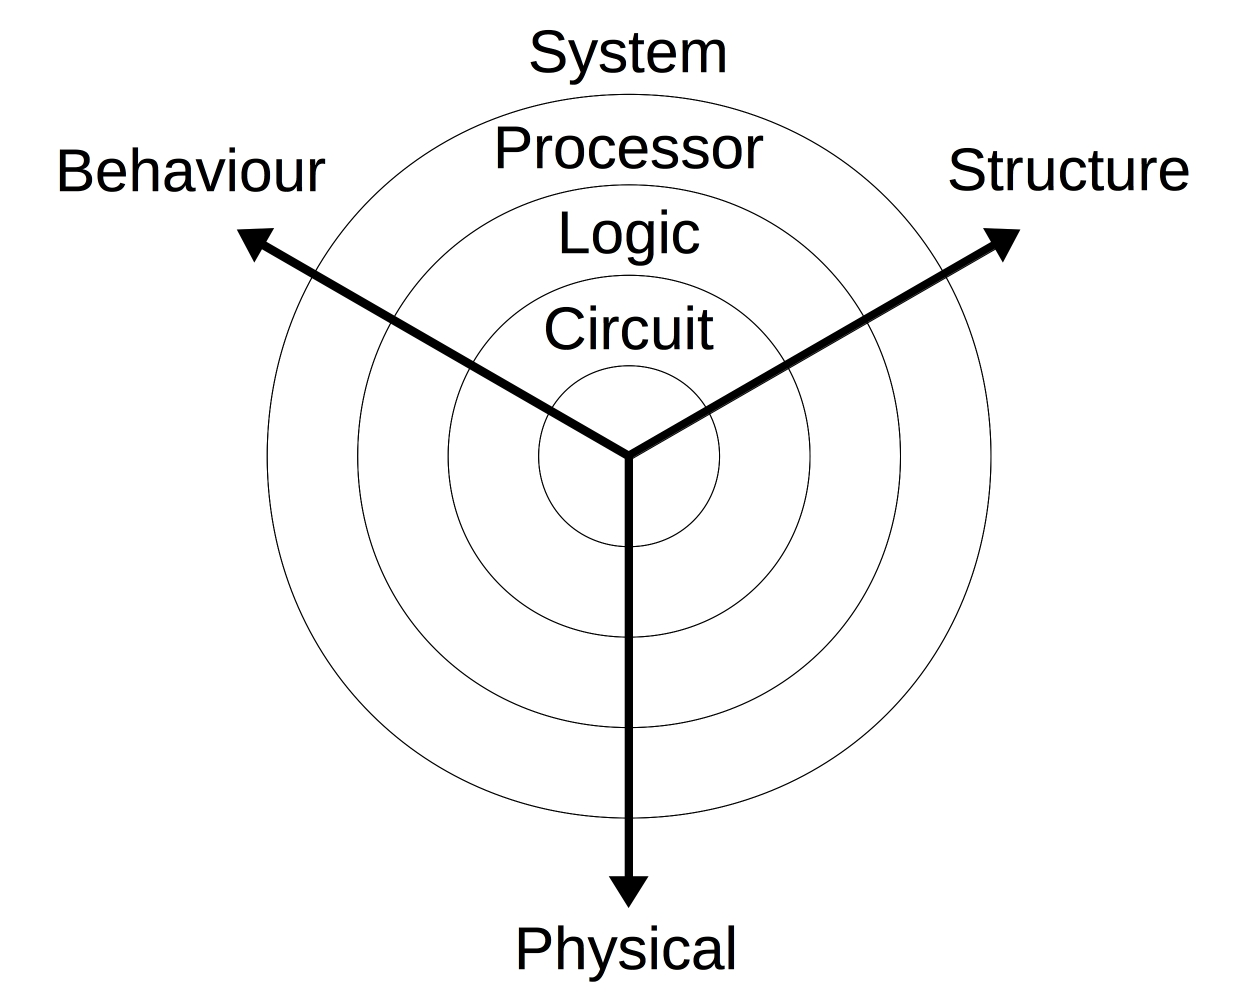
\includegraphics[width=\textwidth]{figures/ychart-std.jpg}
    \caption{Illustration of the standard Gajski-Kuhn Y-chart \cite{gajski2009}\label{fig:ychart_std}}
  \end{subfigure}\hspace{0.25cm}
  \begin{subfigure}[t]{0.475\textwidth}
    \centering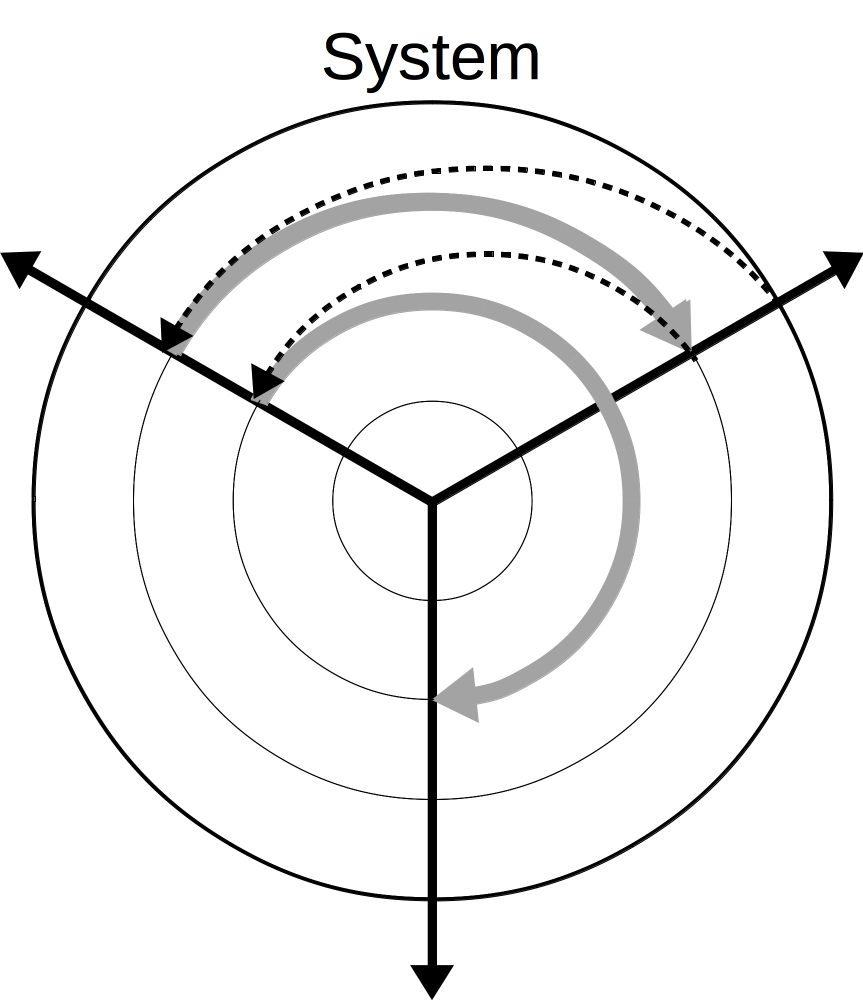
\includegraphics[width=\textwidth]{figures/ychart-fpga.jpg}
    \caption{Illustration of the Gajski-Kuhn Y-chart showing the FPGA methodology \cite{gajski2009}  \label{fig:ychart_fpga}}
  \end{subfigure}\hspace{0.5cm}
  \caption{Illustrations of Gajski-Kuhn Y-chart\label{fig:ychartall}}
\end{figure}

The behavioral domain describes the functional behavior of a system. Going from lowest abstraction level to the higher abstraction level this domain starts being described by transfer functions and at higher levels it will be described by algorithms.\\
The structural domain describes systems using subsystems and their interconnection. Going from the lowest abstraction level to the higher abstraction levels this domain is first described with transistors and at higher levels is will be described using subsystems, FSM, and Data-paths.\\
The physical domain describes how the system is physically put together and is at the lowest levels described using transistor layout and at higher levels it will be described using chips, boards etc.\\

Using the Y-chart for structuring the design process can guide the design process through different design methodology. Two basic methodologies are bottom-up and top-down. \\
The bottom-up methodology starts at the lowest abstraction level and moves through the 3 domains designing the system. Then it goes up a level and uses the results from the lower level to design next level. The bottom-up methodology gives full control of even the smallest details and the final implementation is available earlier. But designing at the lowest abstraction level can quickly be overwhelming and time consuming due to all the details available at the lowest level.\\
Top-down methodology instead starts at the highest abstraction level and designs the system going between the behavioral and structural domains and then go an abstraction level down and at the lowest level the system will be described in physical domain. Since it starts at a higher abstraction level the design process is simpler and it is easier to optimize the system but the cost function for the system is only available in the end of the design process.\\

Another methodology is the FPGA based methodology shown on figure \vref{fig:ychart_fpga} which is a combination of bottom-up and top-down.

%\color{gray}
%\section*{noter til mig selv}
%% --------------------------- udkommentere senere ------
%processor synthesis:\\
%side 32 i gajski pdf \\
%(a) allocation of components and connections \\
%(b) cycle-accurate scheduling\\
%(c) Binding of variables, operations and transfers\\
%(d) Synthesis of controller\\
%(e) Model refinement\\
%(a-c) kan udføres sammen eller i hvilken som helst rækkefølge men de er afhængige af hinanden. Hvis de udføres samtidigt bliver synthesen kompleks og utilregnlig. en strategi er at udføre det i følgende rækkefølge: a c b\\
%Alle trinene ovenover kan udføres automatisk eller manuelt. Hvis det hele bliver udført automatisk kaldes det processor-level synthesis eller high-level synthesis (HLS).  Hvis a-d blvier udført manuelt og e automatisk kaldes det model refinement.\\
%\\
%System-level behavioral model / system synthesis: side 35\\
%(a) Profiling and estimation. \\
%(b) Component and connection allocation\\
%(c) Process and channel binding\\
%(d) Process scheduling\\
%(e) IF component insertion\\
%(f) Model refinement\\
%\\
%1.3 System Design methodology: side 39 \\
%model algebra side 42\\
%algebra:<objects, operations>\\
%$a*(b+c) = a*b+a*c$\\
%dette gør det muligt for system designere at optimere designet vha. arithmetic algebra regler. Udtrykket til venstre for = kræver en multiplier og en adder hvorimod udtrykket på højre side kræver 2 multipliers og en adder.\\
%modelalgebra : <objects, compositions>\\
%\\
%1.4 System-level models: side 44\\
%applications designers, system designers og implementations designers.\\
%\\
%2 system design methodologies side 56\\
%Dette kapitel beskriver forskellige system design methodologies.\\
%Bottom-up: start i bunden (circuit level) kør fra behavior til physical og lav et library. brug dette library til næste level.\\
%Top-down: Start i øverste level (system level) kør fra behavior over til structure. gå et level ned og gentag. ved nederste level gå fra behavior til physical.\\
%Platform methodology: side 61\\
%FPGA methodology: side 64\\
%er based på FPGA substrat som består af multitude af 4-bits ROM celler (Look-up Tables (LUTs)) og disse LUTs kan implementere enhver 4-variable boolsk funktion. I denne design methodologi vil hver RTL kompement in biblioteket være opbygget af disse 4-variable funktioner. Og derefter bliver processor delene synthesizeret af disse RTL componenter.\\
%sagt på en anden måde: denne methodologi bruger en top-down approach på både system og processor levels hvor standard og custom Processing Elements og Communication Elements er opbygget af LUTs. Et system design starter ved at man mapper en applikation ned på en given platform og derefter syntheser brugerdefineret kompenenter ned til RTL komponenter som er defineret in form af LUTs. Standard processor komponenter i processor biblioteket er allerede defineret i form af LUTs. Når alle vores komponenter er defineret vha LUTs så simplificere vi designet ned til LUTs og BRAM og derefter kan vi udføre placering og routing med værktøjer FPGA producentet har udviklet.\\
%Denne form for top-down metode har de samme svagheder som andre top-down metoder som er at det kan være svært at optimere hele designet ved at simplificere designet ned til basiske LUT celler. Derudover ved udvikler heller ikke om hvordan FPGA producentens værktøj placerere og forbinder LUTs og BRAMs.\\
%
%
%\color{black}






